\subsubsection{Flöde vid termisk jämvikt}

\begin{figure}
\centering
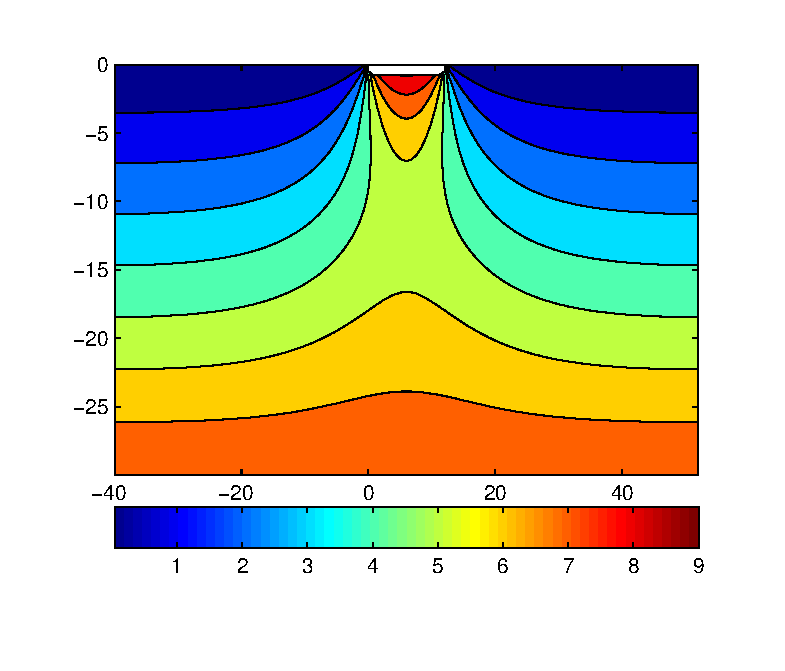
\includegraphics{images/groundheat.eps}
\caption{Temperaturen i marken under en byggnad angivet i grader Celsius. Detta är med termisk jämvikt
med statiska temperaturer och temperaturen långt ner i marken satt till konstanta $\unit[8]{^\circ C}$.}
\end{figure}

\begin{figure}
\centering
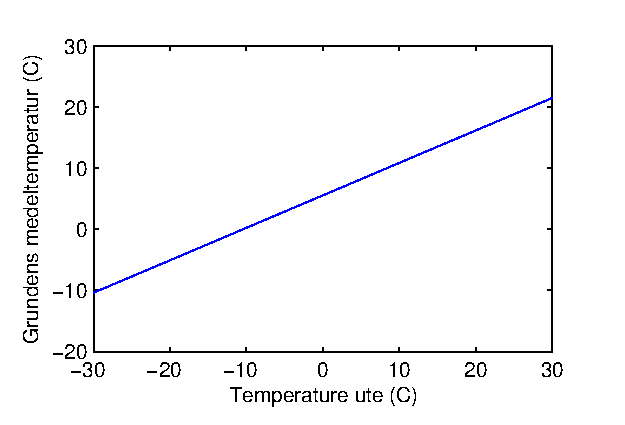
\includegraphics{images/groundtemperature.eps}
\caption{Grundens medeltemperatur mot en referenstemperatur utomhus. Konvektionsparametern är satt till
$h = \unit[15,5]{Wm^{-2}K^{-1}}$.}
\end{figure}
